\section{Auswertung}
\label{sec:Auswertung}

\subsection{Zählrohr-Charakteristik}

Die gemessenen Werte zur Bestimmung der Charakteristik sind in \autoref{tab:messw} zu finden.
\begin{table}[H]
  \caption{Messwerte zur Zählrohr-Charakteristik.}
  \label{tab:messw}
  \centering
  \begin{tabular}{c c c c}
      \toprule
      U [$\si{\volt}$] & N [Imp/$\SI{120}{\second}$] & U [$\si{\volt}$] & N [Imp/$\SI{120}{\second}$] \\
      \midrule
      320 & $ 11680 \pm 108 $ & 520 & $ 12344 \pm 111$ \\
      330 & $ 11939 \pm 109 $ & 530 & $ 12406 \pm 111$ \\
      340 & $ 11946 \pm 109 $ & 540 & $ 12626 \pm 112$ \\
      350 & $ 12320 \pm 111 $ & 550 & $ 12504 \pm 112$ \\
      360 & $ 12291 \pm 111 $ & 560 & $ 12545 \pm 112$ \\
      370 & $ 12371 \pm 111 $ & 570 & $ 12832 \pm 113$ \\
      380 & $ 12393 \pm 111 $ & 580 & $ 12695 \pm 113$ \\
      390 & $ 12433 \pm 112 $ & 590 & $ 12612 \pm 112$ \\
      400 & $ 12259 \pm 111 $ & 600 & $ 12620 \pm 112$ \\
      410 & $ 12157 \pm 110 $ & 610 & $ 12574 \pm 112$ \\
      420 & $ 12428 \pm 111 $ & 620 & $ 12907 \pm 114$ \\
      430 & $ 12475 \pm 112 $ & 630 & $ 12812 \pm 113$ \\
      440 & $ 12566 \pm 112 $ & 640 & $ 12769 \pm 113$ \\
      450 & $ 12440 \pm 112 $ & 650 & $ 12848 \pm 113$ \\
      460 & $ 12645 \pm 112 $ & 660 & $ 12977 \pm 114$ \\
      470 & $ 12446 \pm 112 $ & 670 & $ 13033 \pm 114$ \\
      480 & $ 12625 \pm 112 $ & 680 & $ 13026.\pm 114$ \\
      490 & $ 12516 \pm 112 $ & 690 & $ 13363.\pm 116$ \\
      500 & $ 12415 \pm 111 $ & 700 & $ 13219.\pm 115$ \\
      510 & $ 12632 \pm 112 $ &       &                \\
      \bottomrule
    \end{tabular}
\end{table}

Die Charakteristik ist zusammen mit einer Ausgleichsgeraden für die Werte des Plateau-Bereichs in \autoref{fig:plot} dargestellt. Der Plateau-Bereich wurde hierfür
von $\SI{420}{\volt}$ bis $\SI{560}{\volt}$ gewählt.\\
Da die Werte der Zählrate Poison-verteilt sind, ist ihr Fehler $\Delta N$ als $\sqrt{N}$ anzunehmen.

\begin{figure}[H]
  \centering
  \includegraphics{plot2.pdf}
  \caption{Teilchenanzahl in Abhängigkeit der Spannung.}
  \label{fig:plot}
\end{figure}


Für die Ausgleichsgerade der Form $y = a \cdot x + b$ ergeben sich die Werte
\begin{align*}
  a &= (0,14 \pm 0,5927) \frac{1}{\si{\volt}} \\
  b &= (12434 \pm 291,53)
\end{align*}





Die Plateausteigung ist durch
\begin{equation*}
  N_\text{rel} = \frac{100a}{N(U_\text{m})}
\end{equation*}
gegeben, wobei $U_\text{m}$ als mittlerer Plateauwert gewählt wird.

Der Fehler der Plateausteigung kann über die Gauß'sche Fehlerfortpflanzug zu
\begin{equation*}
  \Delta N_\text{rel} = \sqrt{\left(\frac{100}{N}\symup{\Delta}a\right)^2 + \left(\frac{100a}{N^2} \symup{\Delta}N\right)^2}
\end{equation*}
bestimmt werden.






Daraus ergibt sich eine Plateau-Steigerung von
\begin{align*}
  N_\text{rel} &= \SI{0,11+-0,47}{\percent\per100\volt}
\end{align*}


\subsection{Totzeit}

Zur Bestimmung der Totzeit wurde, wie im vorherigen Abschnitt erwähnt, ein Oszilloskop verwendet. Das Ergebniss ist in \autoref{fig:osz} zu sehen.
\begin{figure}[H]
  \centering
  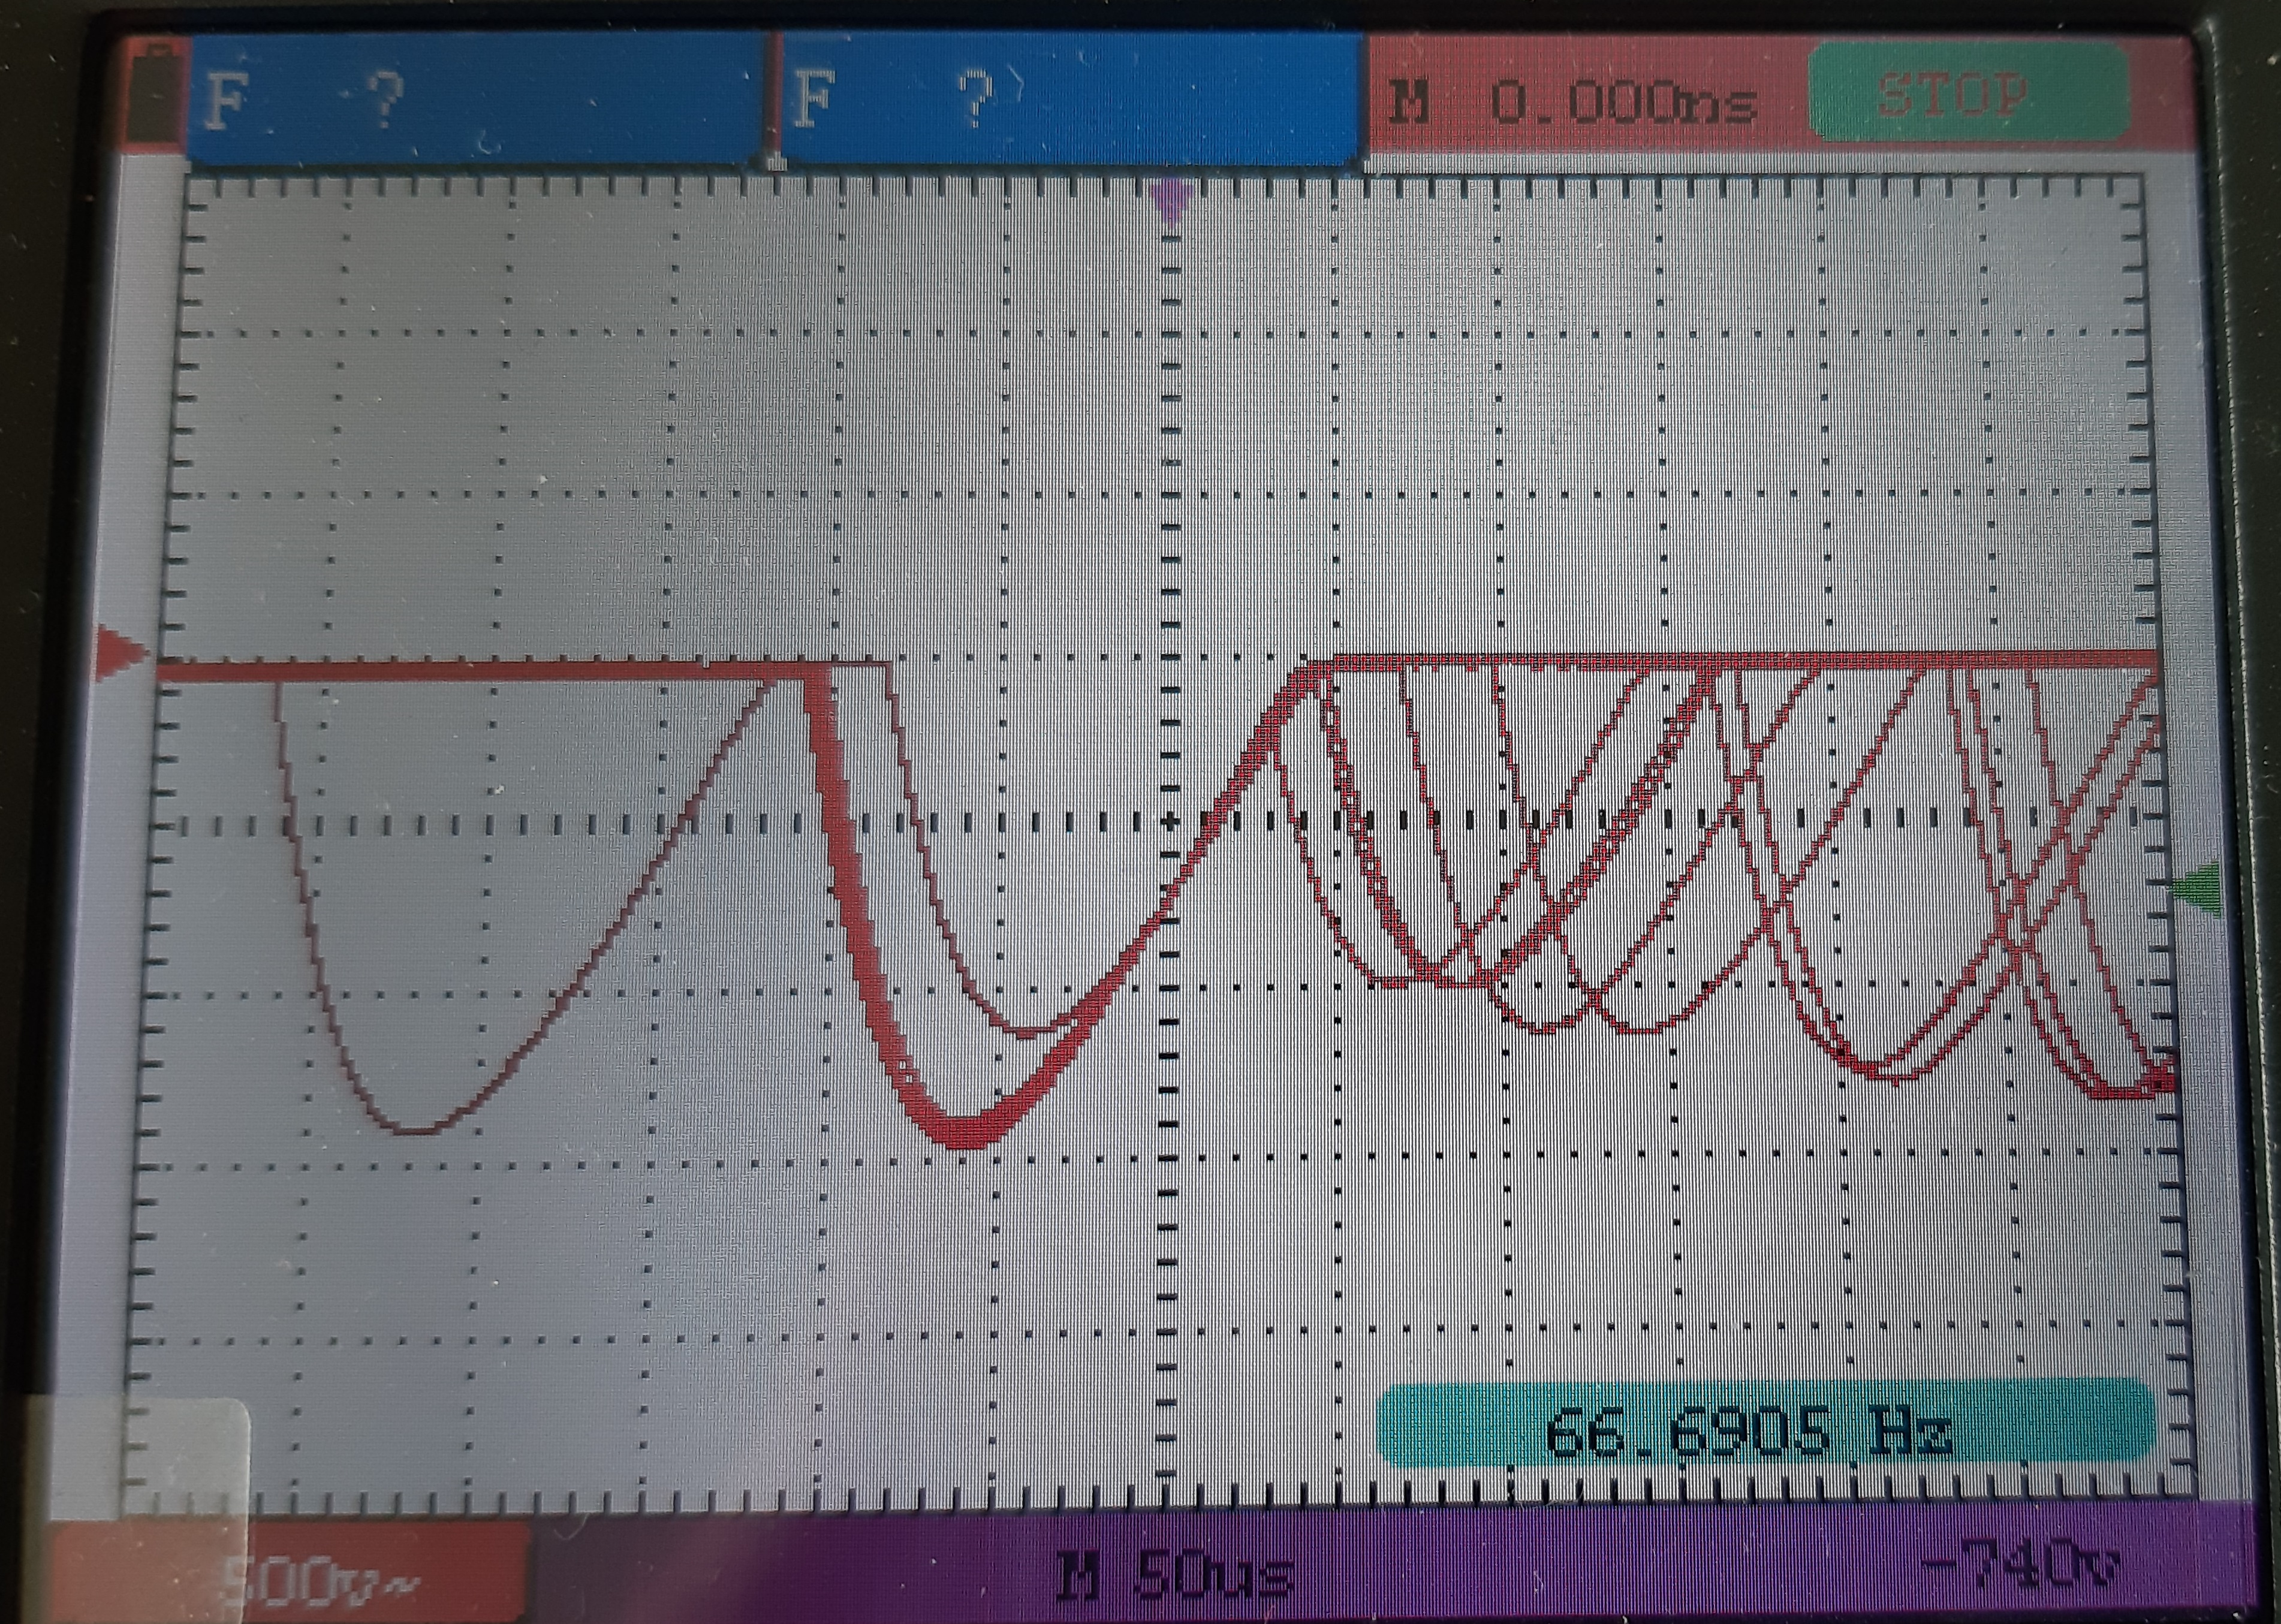
\includegraphics[width=0.7\textwidth]{data/zkurve.jpg}
  \caption{Ergebnisse der Messung mit dem Oszilloskop.}
  \label{fig:osz}
\end{figure}

Die Totzeit kann durch Ablesen bestimmt werden zu
\begin{align*}
  T_\text{t} &= (110 \pm 10) \si{\micro\second}, \\
\end{align*}
die Nachladung zu
\begin{align*}
  T_{n} &= (130 \pm 10) \si{\micro\second}, \\
\end{align*}



Die Totzeit wurde ebenfalls mittels der Zwei-Quellen-Methode bestimmt. Die Ergebnisse der Messungen mit dem ersten Präparat $N_1$, die mit beiden Präparaten
$N_{1+2}$ und die nur mit dem zweiten $N_2$ sind im Folgenden aufgeführt.

\begin{align*}
  N_1 &= 19.344 \pm 139 \\
  N_{1+2} &= 34.387 \pm 185 \\
  N_2 &= 15.440 \pm 124 \\
\end{align*}

Mit Hilfe von Gleichung \eqref{eqn:tot} kann nun die Totzeit zu
\begin{align*}
  T \approx (79,75 \pm 0,30)\si{\micro\second} \\
\end{align*}

bestimmt werden.
Der Fehler wurde dabei mit der Gleichung
\begin{equation*}
  \symup{\Delta}T = \sqrt{\left(\frac{N_1 - N_{1+2}}{2N_2 N_1^2} \cdot \symup{\Delta}N_1 \right)^2 + \left(\frac{N_{1+2} - N_{1}}{2N_1 N_2^2} \cdot \symup{\Delta}N_2 \right)^2
  + \left( \frac{\symup{\Delta}N_{1+2}}{2N_1 N_2}\right)^2} 
\end{equation*}
berechnet.

\subsection{Freigesetzte Ladung pro Teilchen}

Beim Aufnehmen der Messwerte für die Bestimmung der Charakteristik wurden nebenher die jeweils zu den Spannungen zugehörigen Zählrohrströme gemessen. Mit Hilfe von
Gleichung \eqref{eqn:ener} lässt sich daraus die pro Teilchen freigesetze Ladungsmenge $\Delta Q$ berechnen. Die Messwerte sind zusammen mit den errechneten Ladugsmengen in
\autoref{tab:lad} aufgeführt.
\newline
Der Fehler von $\Delta Q$ ist dabei gegene durch
\begin{equation*}
  \Delta (\Delta Q) = \sqrt{\left(\frac{t}{N} \cdot \Delta I \right)^2 + \left(\frac{I \cdot t}{N^2} \cdot \Delta Z\right)^2}.
\end{equation*}

\begin{table}[H]
  \caption{Werte der Regression vom Grad drei.}
  \label{tab:lad}
  \centering
  \begin{tabular}{c c c c c}
      \toprule
      U [$\si{\volt}$] & N [Imp/$\si{\second}$] & I [$\si{\micro\ampere}$] & $\Delta Q$ [$10^9 \si{\coulomb}$] & $10^{10} \frac{\Delta Q}{e}$ \\
      \midrule
      350 & $ 12320 \pm 111 $ & $ 0,2 \pm 0,05 $ & $ 1,95 \pm 0,487 $ & $ 1,22 $ \\
      450 & $ 12440 \pm 112 $ & $ 0,3 \pm 0,05 $ & $ 2,89 \pm 0,483 $ & $ 1,80 $ \\
      540 & $ 12626 \pm 112 $ & $ 0,4 \pm 0,05 $ & $ 3,80 \pm 0,476 $ & $ 2,37 $ \\
      580 & $ 12695 \pm 113 $ & $ 0,5 \pm 0,05 $ & $ 4,73 \pm 0,474 $ & $ 2,95 $ \\
      670 & $ 13033 \pm 114 $ & $ 0,6 \pm 0,05 $ & $ 5,52 \pm 0,463 $ & $ 3,45 $ \\
      700 & $ 13219 \pm 115 $ & $ 0,7 \pm 0,05 $ & $ 6,35 \pm 0,457 $ & $ 3,96 $ \\
      \bottomrule
    \end{tabular}
\end{table}

Nun kann die Ladungsmenge gegen die zugehörige Spannung aufgetragen werden.

\begin{figure}[H]
  \centering
  \includegraphics{plot2.pdf}
  \caption{Ladungsmenge in Abhängigkeit der Spannung.}
  \label{fig:plot}
\end{figure}

Die lineare Regression der Form $y = m \cdot x + b$ liefert die Werte
\begin{align*}
  a &= (12,31 \pm 0,87) \cdot 10^{-3} \si{\coulomb\per\volt} \\
  b &= (-2,54 \pm 0,49) \si{\coulomb}.
\end{align*}
